\documentclass{article}
\usepackage{CJK}
\usepackage{indentfirst}
\usepackage{anysize}
\usepackage{graphicx}
\usepackage{subfigure}
\usepackage{array}
\usepackage{makecell}
\usepackage{url}
\usepackage{float}



%标题缩进
%\usepackage[bf, small]{titlesec}
%    \titleformat{\section}{\bf\large}{\thesection.\,}{0.24em}{}
%    \titlespacing{\section}{0cm}{*1.5}{*1.1}
%    \titleformat{\subsection}{\bf}{\thesubsection.\enspace}{0.5em}{}
%    \titlespacing{\subsection}{15pt}{*1.5}{*1.1}
%    \titleformat{\subsubsection}{}{\thesubsubsection.\,}{0.24em}{}
%    \titlespacing{\subsubsection}{30pt}{*1.5}{*1.1}

\usepackage{listings}
\usepackage{color}

\definecolor{dkgreen}{rgb}{0,0.6,0}
\definecolor{gray}{rgb}{0.5,0.5,0.5}
\definecolor{mauve}{rgb}{0.58,0,0.82}

\lstset{ %
  language=C++,                % the language of the code
  basicstyle=\footnotesize,           % the size of the fonts that are used for the code
  numbers=left,                   % where to put the line-numbers
  numberstyle=\tiny\color{gray},  % the style that is used for the line-numbers
  stepnumber=2,                   % the step between two line-numbers. If it's 1, each line 
                                  % will be numbered
  numbersep=5pt,                  % how far the line-numbers are from the code
  backgroundcolor=\color{white},      % choose the background color. You must add \usepackage{color}
  showspaces=false,               % show spaces adding particular underscores
  showstringspaces=false,         % underline spaces within strings
  showtabs=false,                 % show tabs within strings adding particular underscores
  frame=single,                   % adds a frame around the code
  rulecolor=\color{black},        % if not set, the frame-color may be changed on line-breaks within not-black text (e.g. commens (green here))
  tabsize=2,                      % sets default tabsize to 2 spaces
  captionpos=b,                   % sets the caption-position to bottom
  breaklines=true,                % sets automatic line breaking
  breakatwhitespace=false,        % sets if automatic breaks should only happen at whitespace
  title=\lstname,                   % show the filename of files included with \lstinputlisting;
                                  % also try caption instead of title
  keywordstyle=\color{blue},          % keyword style
  commentstyle=\color{dkgreen},       % comment style
  stringstyle=\color{mauve},         % string literal style
  escapeinside={\%*}{*)},            % if you want to add LaTeX within your code
  morekeywords={*,...}               % if you want to add more keywords to the set
}


\linespread{1.5}


\marginsize{3.5cm}{3.5cm}{2cm}{2cm}
\setlength{\parindent}{2em}

\newcolumntype{L}[1]{>{\vspace{0.5em}\begin{minipage}{#1}\raggedright\let\newline\\
\arraybackslash\hspace{0pt}}m{#1}<{\end{minipage}\vspace{0.5em}}}
\newcolumntype{R}[1]{>{\vspace{0.5em}\begin{minipage}{#1}\raggedleft\let\newline\\
\arraybackslash\hspace{0pt}}m{#1}<{\end{minipage}\vspace{0.5em}}}
\newcolumntype{C}[1]{>{\vspace{0.5em}\begin{minipage}{#1}\centering\let\newline\\
\arraybackslash\hspace{0pt}}m{#1}<{\end{minipage}\vspace{0.5em}}}


%使得图片显示对应章节
\renewcommand\thefigure{\thesection.\arabic{figure}}
\makeatletter
\@addtoreset{figure}{section}
\makeatother

\begin{document} 
\begin{CJK}{UTF8}{gbsn}

\newcommand*{\titleGP}{\begingroup % Create the command for including the title page in the document
\centering % Center all text
\vspace*{\baselineskip} % White space at the top of the page

\rule{\textwidth}{1.6pt}\vspace*{-\baselineskip}\vspace*{2pt} % Thick horizontal line
\rule{\textwidth}{0.4pt}\\[\baselineskip] % Thin horizontal line

{\LARGE 请求调页存储管理方式模拟
 \\ \vspace{2em} \begin{large} 操作系统课程设计 \end{large}}\\[0.2\baselineskip] % Title

\rule{\textwidth}{0.4pt}\vspace*{-\baselineskip}\vspace{3.2pt} % Thin horizontal line
\rule{\textwidth}{1.6pt}\\[\baselineskip] % Thick horizontal line

\scshape % Small caps
%利用操作系统中的多线程思想,自我实现电梯调度算法 \\[\baselineskip] % Tagline(s) or further description
operating system,  Spring 2017\par % Location and year

\vspace*{2\baselineskip} % Whitespace between location/year and editors

 By \\[\baselineskip]
{\Large1552674 李源 \par} % Editor list


\vfill % Whitespace between editor names and publisher logo

{\itshape Tongji University \\ School of Software Engineering \par}

\endgroup}


\titleGP % This command includes the title page
\clearpage
\tableofcontents
\clearpage

\section{项目背景}
\subsection{项目需求}
编写一个应用程序,实现请求调页存储管理方式模拟。假设每个页面可存放10条指令,分配给一个作业的内存块为4。模拟一个作业的执行过程,该作业有320条指令,即它的地址空间为32页,目前所有页还没有调入内存。采用FIFO算法或LRU算法实现置换。指令分布应该是均匀的。

\subsection{项目目的}
(1) 掌握页面、页表、地址转换过程;

(2) 对页面置换过程有更深的认识;

(3) 加深对请求调页系统的原理和实现过程的理解。


\vspace{4em}

\section{需求分析}
根据项目需求,我们可以得知本项目所模拟的内存和作业分别满足如下要求:

(1) 内存:4个内存块,一个内存块中能存放10条指令;

(2) 作业:320条指令,分别放在32页中;需执行320条指令,且指令可以重复。

(3) 指令分布:50\%的指令是顺序执行的,25\%是均匀分布在前地址部分,25\%是均匀分布在后地址部分。

(4) 置换算法:分别实现LRU算法和FIFO算法。


结合内存和作业的实际情况,我们可以设计出本项目的模拟方案。

\subsection{模拟方案}
该模拟方案的步骤,大致可按照如下进行:

(1) 随机从一条指令开始执行。

(2) 如果指令在内存中,则显示其物理地址,并转到下一条指令;如果不在不在内存中,则发生缺页,此时需要记录缺页次数,并将其调入内存。

(3) 如此循环,直到执行了320条指令,之后不再执行。


\clearpage

\section{调度算法}
根据前文对本模拟系统的分析,以及对两种指令情况的具体考虑,可以将该调度算法细分为两个部分:

(1) 实现内存块的置换算法,即LRU算法和FIFO算法;

(2) 实现指令的随机选择算法,可称为random算法。

\subsection{FIFO算法}
根据FIFO算法的定义,最先进来的页,最先被调出。则FIFO算法的关键是,将调入的页以队列的数据结构形式存储,利用队列实现先入先出。在本模拟系统中,我使用一个数组完成FIFO算法中队列的实现。FIFO算法的步骤如下:

(1) 该数组存储四个内存块进入的顺序。

(2) 初始化的时候,该数组所有的值被初始化为0。

(3) 每次执行指令时,首先检测该指令是否在某一个内存块中。

(4) 如果在某一个内存块中,则没有任何操作。

(5) 如果不在内存块中,首先查找是否有内存块为空,如果空,就放入其中。

(6) 如果没有内存块为空,则选择内存块时间为4的那一个,将其替换,替换后时间改为0,其余的内存块时间加1。

\begin{figure}[!h]
\centering
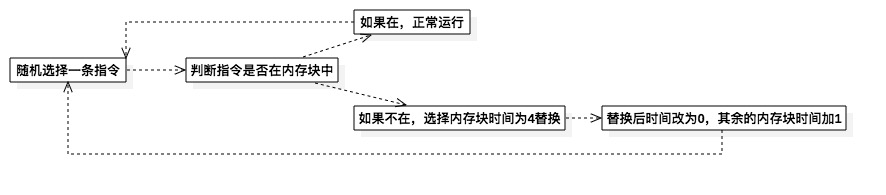
\includegraphics[width=1.1\textwidth]{1.jpg}
\caption{FIFO算法示意图}
\end{figure}

\subsection{LRU算法}
根据LRU算法的定义,使用离过去最近作为不远将来的近似,将最长时间没有使用的页置换出去。则LRU算法的关键是,选择最长时间没有使用的页,并且置换出去。在本模拟系统中,我使用一个数组完成LRU算法中对于最长时间没有使用的页寻找。LRU算法的步骤如下:

(1) 该数组存储四个内存块各自上次使用的时间。

(2) 初始化的时候,该数组所有的值被初始化为0。

(3) 每次执行指令时,首先检测该指令是否在某一个内存块中。

(4) 如果在某一个内存块中,将其该内存块的时间改为0,其余的内存块时间加1。

(5) 如果不在内存块中,找到4个内存块中时间最大的那一个,将其替换,替换后时间改为0,其余的内存块时间加1。

\begin{figure}[!h]
\centering
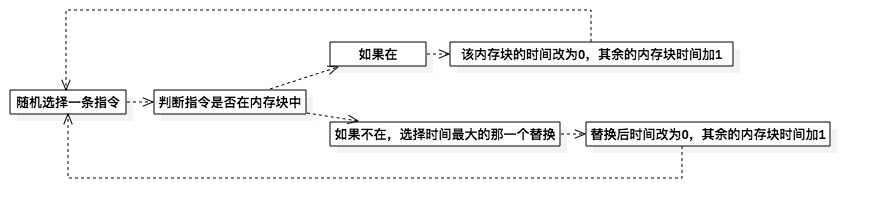
\includegraphics[width=1.1\textwidth]{2.jpg}
\caption{LRU算法示意图}
\end{figure}

\subsection{指令随机选择算法}
本算法以ppt给出的参考方法为标准,具体步骤如下:

(1) 在0至319条指令之间,随机选取一个起始执行指令。如序号为$m$。

(2) 顺序执行下一条指令,即序号为$m+1$的指令。

(3) 通过随机数,跳转到前地址部分0 至$m-1$中的某个指令处,其序号为$m_{1}$。

(4) 顺序执行下一条指令,即序号为$m_{1}+1$的指令。

(5) 通过随机数,跳转到后地址部分$m_{1}+2$至319中的某条指令处,其序号为$m_{2}$。

(6) 顺序执行下一条指令,即$m_{2}+1$处的指令。

(7) 重复跳转到前地址部分、顺序执行、跳转到后地址部分、顺序执行的过程,直到执行完320条指令。

其中随机数的生成,利用qsrand函数实现,具体代码如下:

\begin{lstlisting}
QTime t;
t= QTime::currentTime();
qsrand(t.msec()+t.second()*1000);

int temp = qrand() % this->nowAchieve;
int temp = this->nowAchieve + qrand() % (319 - this->nowAchieve);
	
\end{lstlisting}
\clearpage

\section{系统实现}
根据需求分析,可以将该模拟系统的界面分为2个部分,分别为控制界面和显示界面。如下:

\begin{figure}[!h]
\centering
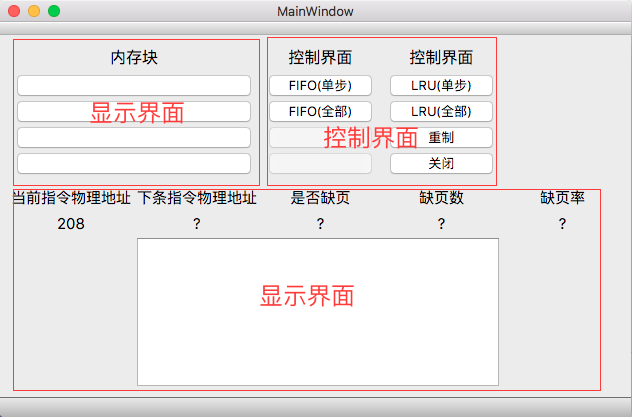
\includegraphics[width=0.8\textwidth]{3.png}
\caption{系统界面图}
\end{figure}

\subsection{控制界面}
控制界面可选择不同的算法,"单步"表示执行一条指令,"全部"表示一次性执行完所有指令。本轮320条指令执行完后,或中途想重新开始,均可点击"重制"按钮重新开始。点击"关闭"按钮退出本模拟系统。注意,在使用一种算法后,中途不可切换算法。
\begin{figure}[!h]
\centering
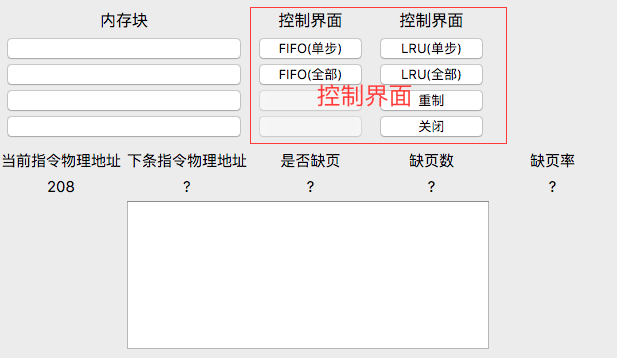
\includegraphics[width=0.8\textwidth]{4.png}
\caption{控制界面图}
\end{figure}

\clearpage
\subsection{显示界面}
显示界面可分为两部分,即内存块部分和指令部分。
\begin{figure}[!h]
\centering
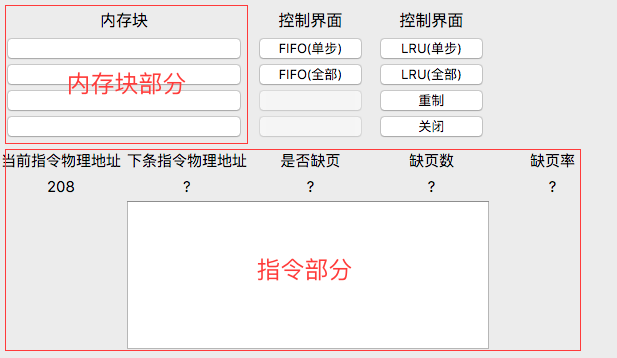
\includegraphics[width=0.55\textwidth]{5.png}
\caption{显示界面图}
\end{figure}

其中内存块部分,当某一个内存块放入了某一页后,内存块会变为"已满"的状态,且显示当前放入的逻辑页号。
\begin{figure}[!h]
\centering
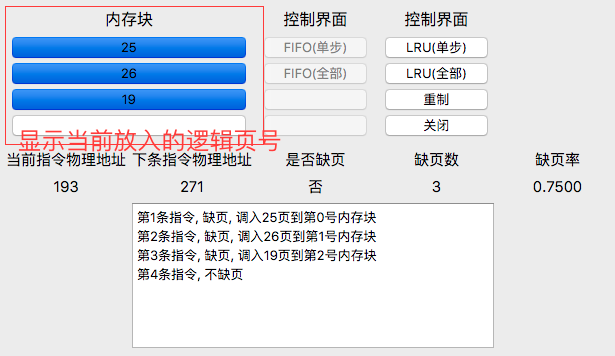
\includegraphics[width=0.55\textwidth]{6.png}
\caption{内存块部分}
\end{figure}

而指令部分,会显示当前与下一条指令地址,当前是否出现缺页情况,总的缺页数和缺页率。同时,也可在下面查看之前的指令相关信息。
显示界面可分为两部分,即内存块部分和指令部分。
\begin{figure}[!h]
\centering
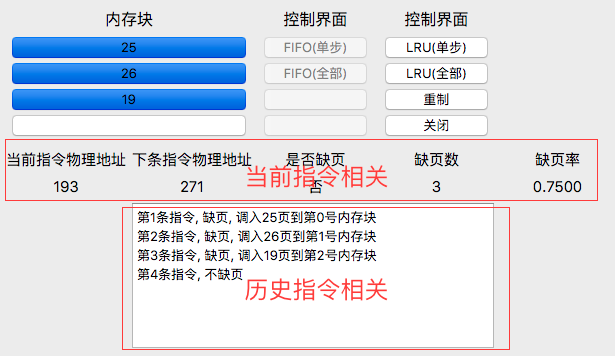
\includegraphics[width=0.55\textwidth]{7.png}
\caption{指令部分}
\end{figure}

\clearpage
\subsection{LRU算法与FIFO算法区别}
由于本模拟系统所使用的指令随机选择算法原因,两个算法在缺页数和缺页率上的差别并不明显,其主要的差异在于,使用FIFO算法时,被替换的内存块始终按照同一顺序,如本例的0-1-2-3。而LRU算法则会没有特定的顺序。这一区别是因为其算法本质而产生的。效果如下:
\begin{figure}[!h]
  \subfigure[FIFO算法]{
    \label{fig:subfig:a} %% label for first subfigure
    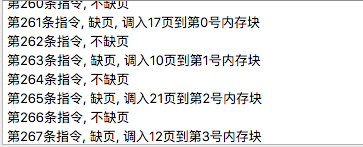
\includegraphics[width=0.45\textwidth]{8.PNG}}
  \hspace{0.5in}
  \subfigure[LRU算法]{
    \label{fig:subfig:b} %% label for second subfigure
    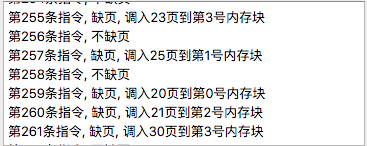
\includegraphics[width=0.45\textwidth]{9.PNG}}
   
  \caption{两者算法区别}
  \label{fig:subfig} %% label for entire figure
 \end{figure}

\vspace{3em}
\section{开发环境}
\begin{itemize}
	\item 系统:macOS Sierra (version 10.12.5)
	\item IDE:Qt Creator 4.2.1, Based on Qt 5.8.0 (Clang 7.0 (Apple), 64 bit)
	\item 语言: C++
\end{itemize}

\vspace{3em}
\section{提交内容}
\begin{itemize}
	\item 源代码
	\item assignment2.zip 可执行文件压缩包(需在mac系统下使用)
	\item assignment2.dmg 安装包(需在mac系统下使用)
	\item 1552674\_liyuan.pdf 说明文档
\end{itemize}

\end{CJK}
\end{document}